\subsection{Introduction}
\label{sec:kpimm:introduction}

The decay \BdToKpimm is a rare, FCNC process that proceeds through electroweak penguin or box diagrams in the SM. In extensions to the SM, new heavy particles can enter the loop and modify observables such as branching fractions and kinematic distributions of the final state particles. 

The previous analyses of \BdToKpimm performed by the \lhcb collaboration~\cite{kstmm-0.3fb,kstmm-1fb,kstmm-1fb-pprime,kstmm-3fb} have focused on the $796<\mkpi<996~\mevcc$ region where the $\kaon\pion$ comes predominately from the P-wave decay $\decay{\Kstarone(892)}{K\pi}$. In this region, the differential branching fraction has been measured along with several different sets of angular observables.

While the observables measured in~\cite{kstmm-0.3fb,kstmm-1fb} were largely in agreement with SM predictions, a 3.7$\sigma$ local deviation was seen in the observable $P_{5}^{'}$~\cite{kstmm-1fb-pprime}. This deviation was later confirmed by an updated measurement~\cite{kstmm-3fb}. The two results are shown in Fig.~\ref{fig:kpimm:p5prime}. 

\begin{figure}[!tb]
\centering
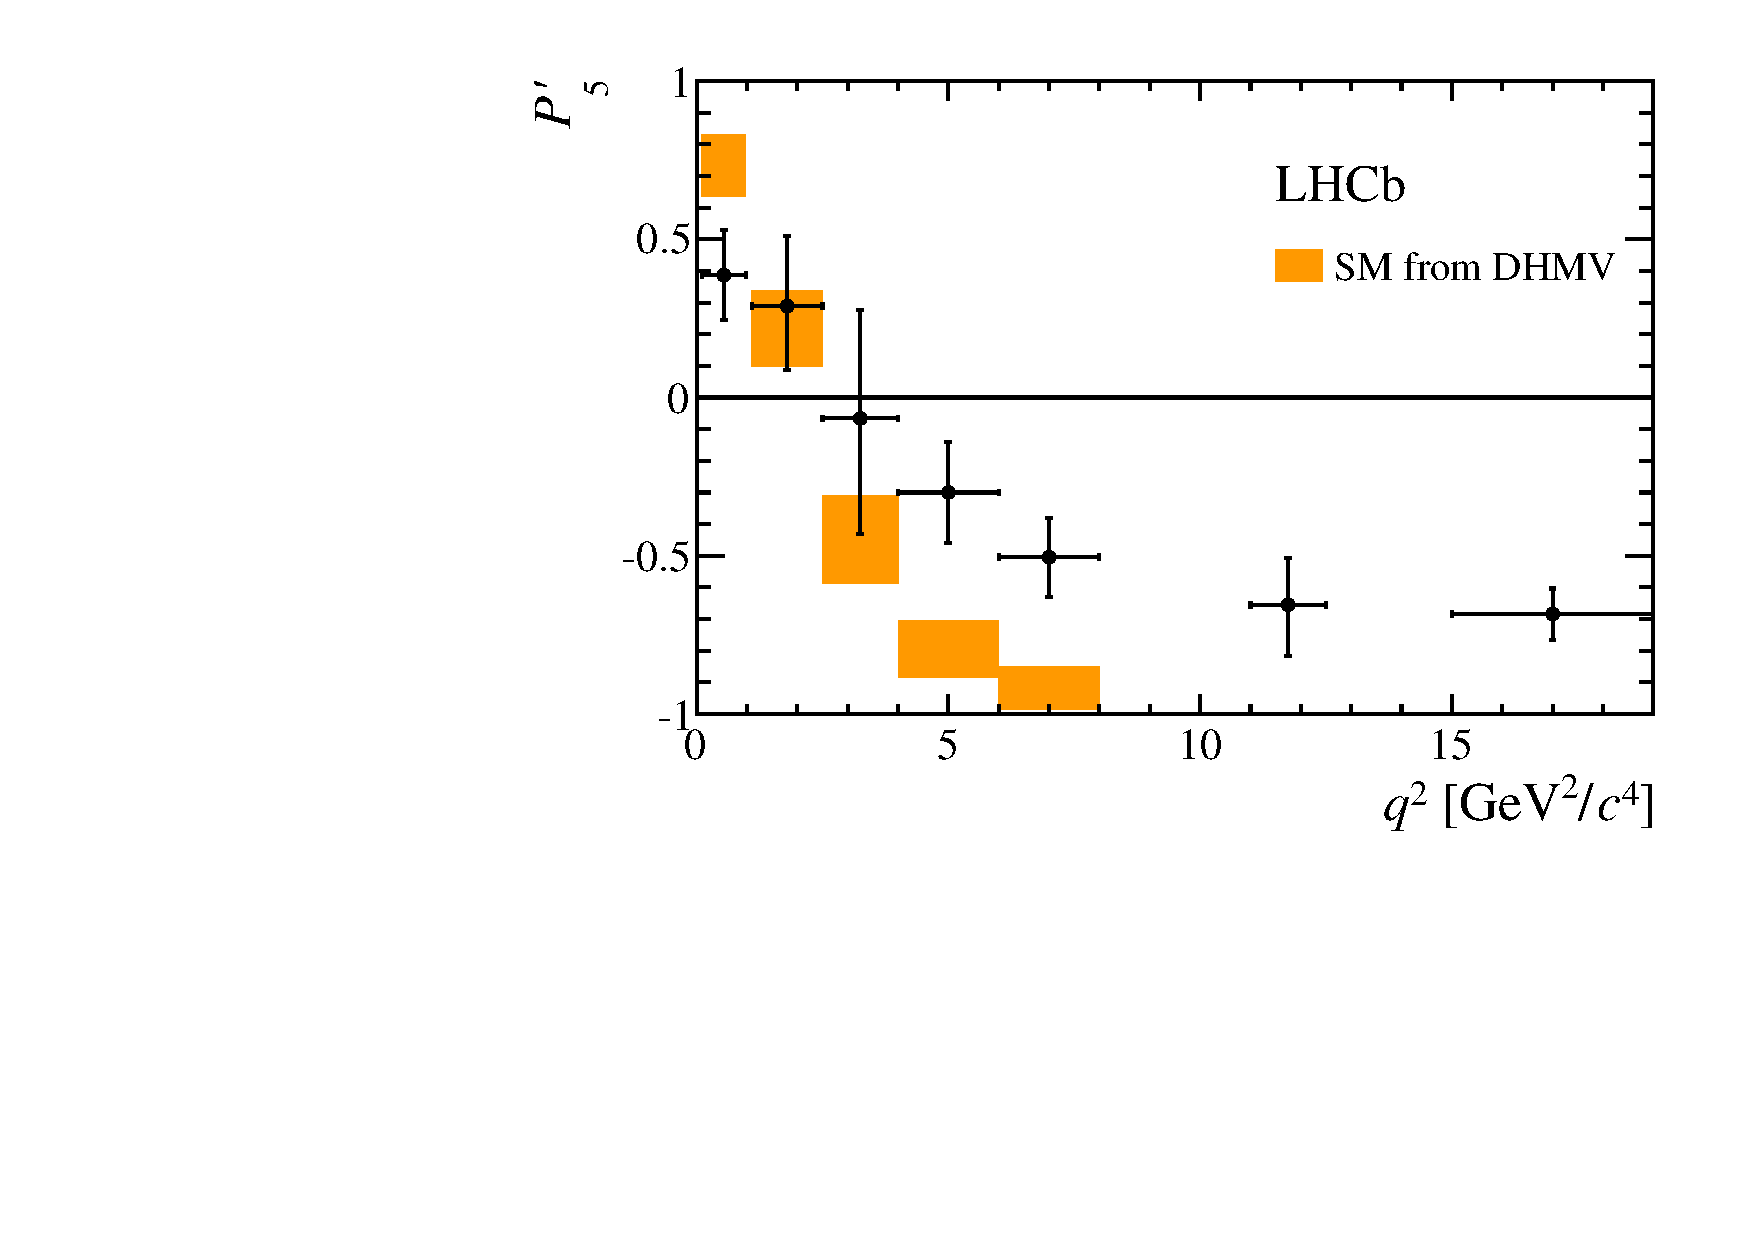
\includegraphics[width=0.8\textwidth]{figs/kpimm/introduction/P5prime.pdf}
\caption{Results of the measurement of the observable $P_{5}^{'}$ by the \lhcb collaboration. The SM predictions are taken from~\cite{pprime-theory}.}
\label{fig:kpimm:p5prime}
\end{figure}

As shown in Tab.~\ref{tab:introduction:states}, the previously unexplored $1330<\mkpi<1530~\mevcc$ region contains contributions from $S$-, $P$- and $D$-waves. The goal of the following analysis is to measure the differential branching fraction and perform an angular analysis of \BdToKpimm in this \mkpi range.
 
\begin{table}[!tb]
\centering
\caption{Known \KstarJ states that can contribute to \BdToKpimm over the \mkpi range of interest in this analysis. The numerical values are taken from~\cite{pdg}.} 
\begin{tabular}{c|c|c|c|c}
   & $J^{P}$ & Mass~[\mevcc] & Full width~[\mevcc]  & $\Gamma_{K\pi}/\Gamma~[\%]$ \\
  \hline
  \Kstarone(1410) & $1^{-}$& $1414 \pm 15$& $232 \pm 21$  & 6.6 $\pm$ 1.3 \\
  \Kstarzero(1430) & $0^{+}$ & $1425 \pm 50$ & $270 \pm 80$ & 93 $\pm$ 10 \\
  \Kstartwo(1430) & $2^{+}$ & $1432.4\pm 1.3$ & $109 \pm 5$ & 49.9 $\pm$ 1.2 \\
  %\Kstarone(1680) & $1^{-}$ & $1717 \pm 27$ & $322 \pm 110$ & 38.7 $\pm$ 2.5 \\
  %\Kstarthree(1780) & $3^{-}$ & $1776 \pm 7$ & $159 \pm 21$ & 18.8 $\pm$ 1.0 \\
  %\Kstarfour(2045) & $4^{+}$ & $2045 \pm 9$ & $198 \pm 30$ & 9.9 $\pm$ 1.2 \\
\end{tabular}
\label{tab:introduction:states}
\end{table}